
\subsection{Training on more trials with skip memory enables many-shot adaptation} \label{sec:results_few_to_many_shot}

So far, we have considered the few-shot regime in which we train on 1 to 6 trials and evaluate up to 13 trials. In this section, we evaluate AdA's ability to adapt over longer time horizons. We find that when trained with $k \in \{1, 2, \dots 6\}$, agents do not continue to adapt past 13 trials; however, this long-term adaptation capability is greatly improved by increasing the maximum number of trials during training to 24 and increasing the effective length of the memory accordingly. These results show that our method naturally extends to many-shot timescales, with episodes lasting in excess of $30$ minutes.\footnote{$48$ trials of a $40$s task lasts for 32 minutes. By contrast, the average length of a Starcraft 2 game is between $10$ and $15$ minutes, and AlphaStar acted less frequently per-second than AdA does \citep{alphastar}.} In this section, we ablate both factors separately, and show that both are important for long-range adaptation. The training configuration (which is identical to that of the memory scaling experiments save for the number of training steps) is detailed in Table \ref{tab:skip-memory-scaling}.

As we noted in Section \ref{sec:scaling_results}, increasing the memory length leads to increased capacity that benefits the agent even when the entire episode fits in memory, but also comes at the cost of increased computation. To disentangle these factors, we propose a simple change to the memory architecture described in Section \ref{sec:memory-architectures} which increases effective memory length without increasing computational cost. We use a GRU to encode trajectories before feeding them to the Transformer-XL. This allows us to sub-sample timesteps from the encoded trajectories, enabling the agent to attend over 4 times as many trials without additional computation. We show that the additional GRU on its own does not affect the performance of the agent greatly.

As can be seen in Figure~\ref{fig:manyshot_ablation}, increasing the number of trials in the training distribution significantly boosts performance in later trials, especially when the memory length is scaled accordingly. In other words, the adaptation strategy learned by AdA benefits from experiencing a large number of trials, rather than just very recent ones. Therefore we can conclude that AdA is capable of adaptation based on long-term knowledge integrated into memory across many trials, as opposed to merely encoding a simple meta-strategy that only depends on the trajectory from the previous trial.  

Increasing the number of trials in training leads to better adaptation even in the absence of increased memory. This indicates that the agent is able to learn better exploration and refinement strategies when afforded longer training episodes consisting of more trials. Note that increasing effective memory without increasing the number of training trials does not improve performance, as the agent has not been trained to make use of the additional memory capacity.

\begin{figure}[t]
    \centering
    \begin{subfigure}{0.49\textwidth}
    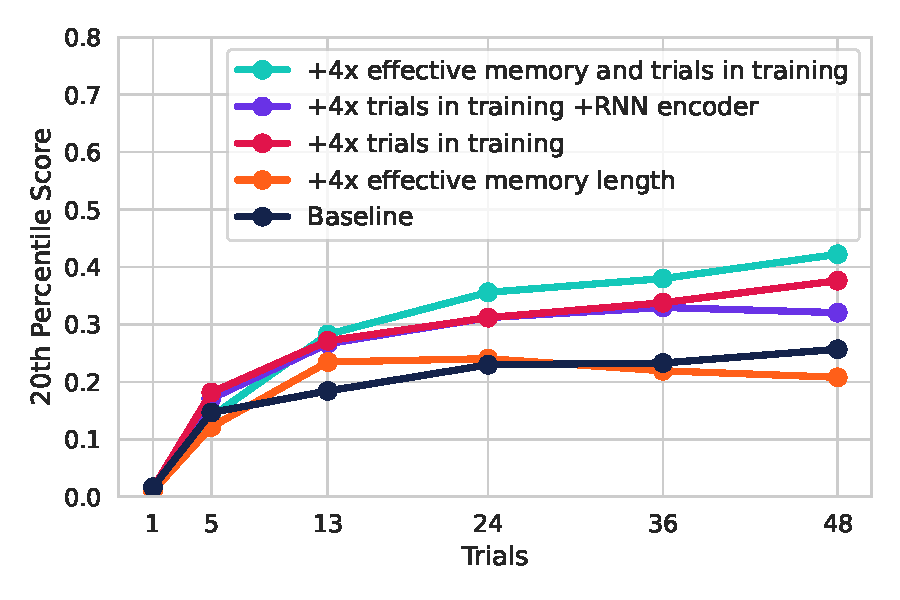
\includegraphics[width=\linewidth]{figures/manyshot_ablation.pdf} 
     \vskip -3pt \caption{}
    \label{fig:manyshot_ablation}
    \end{subfigure}
    \begin{subfigure}{0.49\textwidth}
    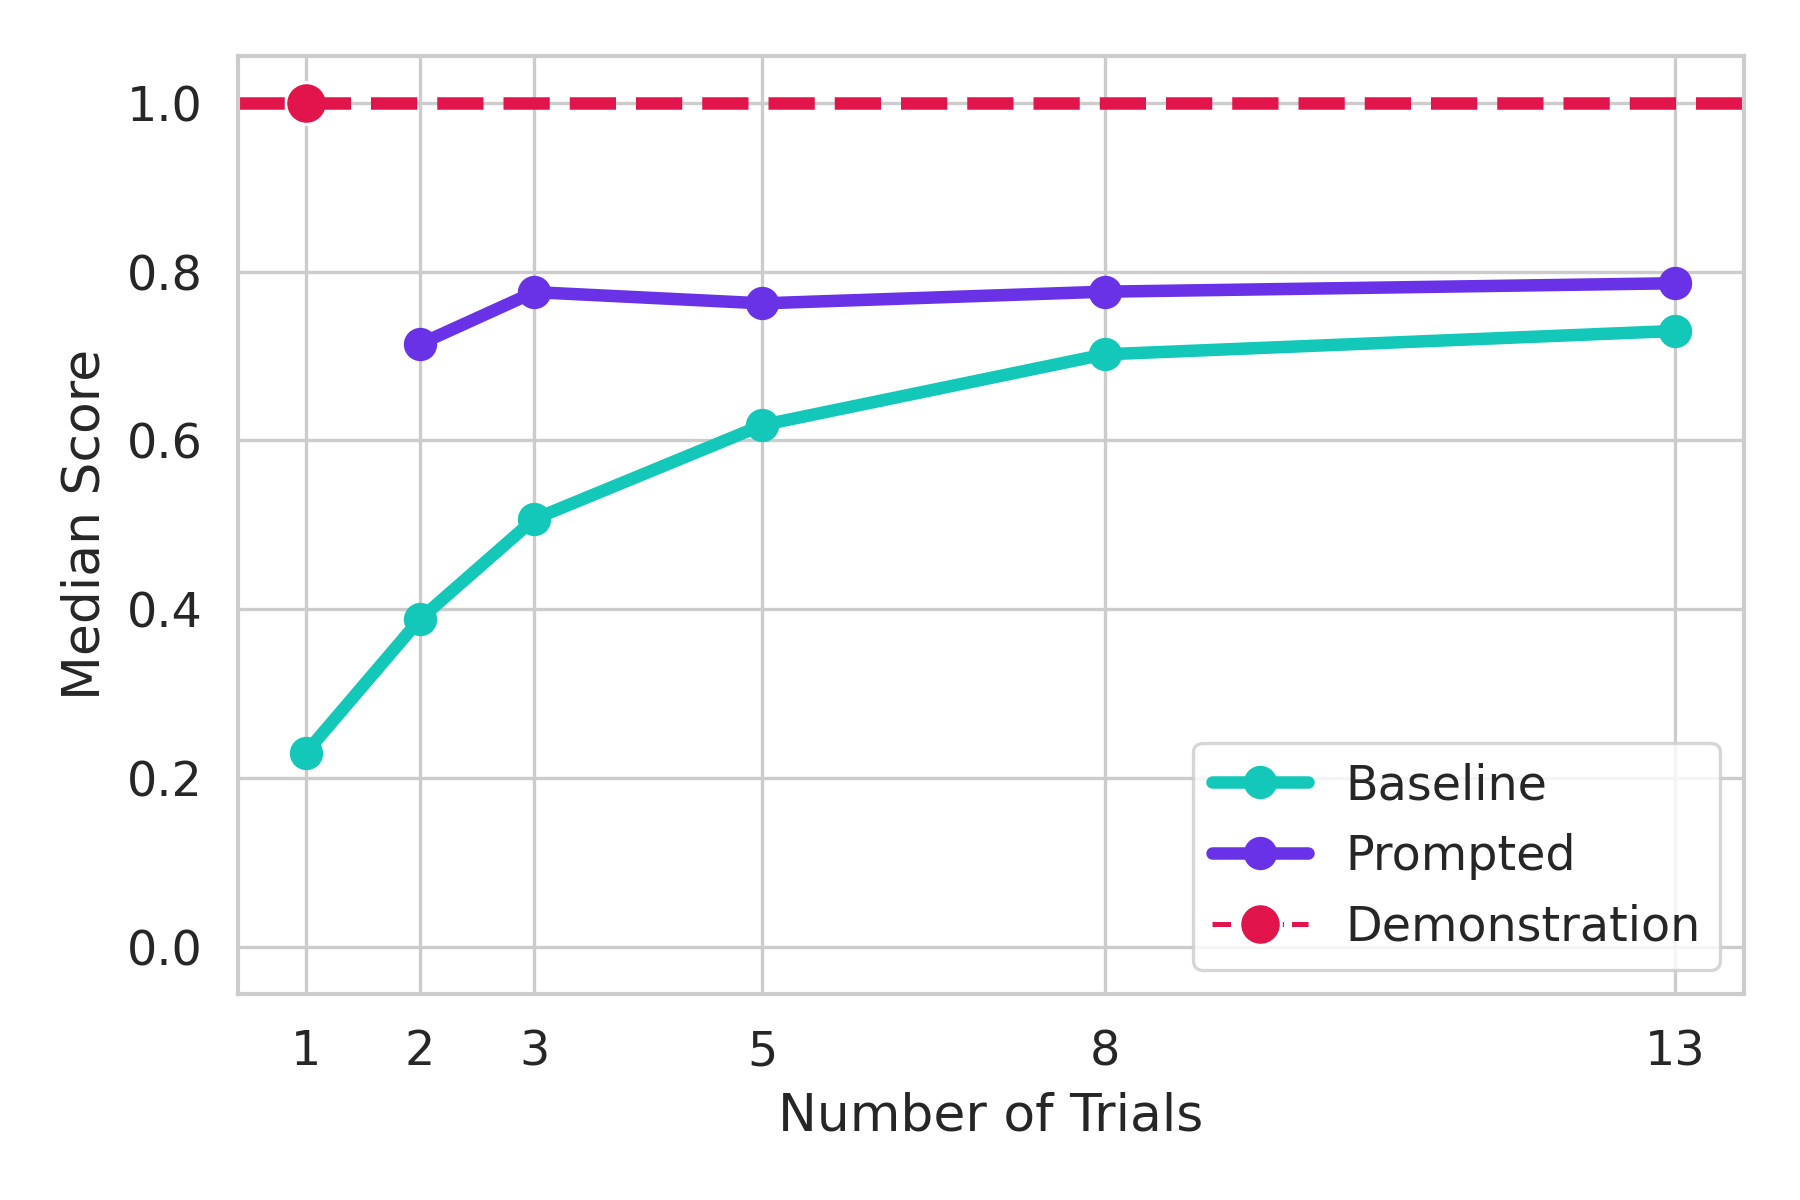
\includegraphics[width=\linewidth]{figures/first-person-demonstration.png}
     \vskip -3pt \caption{}
    \label{fig:first-person-demonstration}
    \end{subfigure}
    \caption{\textbf{(a)} Ablation showing the 20\textsuperscript{th} percentile of test scores as we vary the maximum number of training trials (from a $k=6$ baseline to $k=24$) and increase the effective memory size via sub-sampling (from 1800 steps to 7200 steps). Together, these factors enable the agent to adapt over a larger number of trials (lasting over 30 minutes). Increasing the number of training trials has the biggest effect and is a prerequisite for sub-sampling to be effective. This figure furthermore shows that adding an RNN encoder to facilitate sub-sampling does not by itself greatly affect performance. \textbf{(b)} Median hand-authored task score of AdA prompted with a first-person demonstration in the first trial of each episode, compared with an unprompted baseline. The prompted score lies strictly above the baseline which indicates that AdA is able to use information from a demonstration prompt to improve its performance. However, the score lies below that of the demonstration which suggests that it is not able to make perfect use of the demonstration.}
\end{figure}

